% Drawing 138/06-48 -- folder 138, batch 06, archive page 118 (PDF page 119).
% Transcription: une croix à deux sommets terminaux, $\mathbb{Z}_2$ ; une boucle avec deux arêtes à sommets terminaux, $\mathbb{Z}_2$ ; $(\delta)$ une croix à deux sommets opposés, $\mathbb{Z}_2 \times \mathbb{Z}_2$ ; $(\eta)$ un cercle avec un rayon prolongé, $\mathbb{Z}_2$.
% Kind: table of small maps with automorphism groups (degree 6, d). Method 2 (schematic redraw from the facsimile). Status: ok.
% Notes: d): a cross with two terminal vertices, Z_2; a loop with two edges ending at vertices, Z_2; (delta) a cross with two opposite vertices, Z_2 x Z_2; (eta) a circle with a ray prolonged, Z_2 (the last two smaller, in another ink). Each small map carries its automorphism group as written (given as labels, since the transcription names them); vertex positions and loop shapes approximate.
% Coordinates: 1 unit = 1 mm = 1/100 of the crop width (bbox in page fractions: [0.231, 0.62, 0.769, 0.739]).
% Redrawn by Claude (claude-opus-5-5), issue #73, 2026-11-07; not checked by a human; not compiled (no TeX in the session).
% Rights: reproduces part of the work -- behind RENDER_TRANSCRIPTS, never published by itself.
\documentclass[tikz,border=3pt]{standalone}
\usepackage{amsmath,amssymb}
\usetikzlibrary{patterns,arrows.meta}
\tikzset{pencil/.style={black!45}, struck/.style={black!35}, mark/.style={circle,draw,inner sep=1.3pt}, pt/.style={circle,fill,inner sep=0.9pt}, opt/.style={circle,draw,fill=white,inner sep=1.1pt}}
\begin{document}
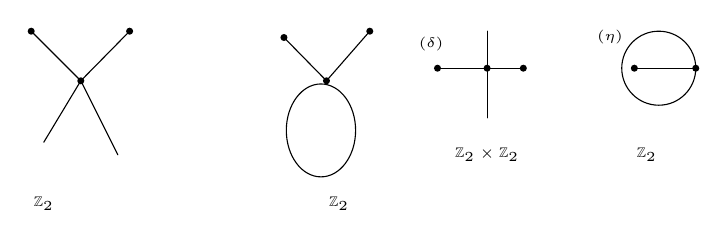
\begin{tikzpicture}[x=1mm,y=1mm,line cap=round,line join=round,font=\scriptsize]
\draw (17.2,-12.5) -- (10.9,-6.2);
\draw (17.2,-12.5) -- (23.4,-6.2);
\draw (17.2,-12.5) -- (12.5,-20.3);
\draw (17.2,-12.5) -- (21.9,-21.9);
\node[pt] at (17.2,-12.5) {};
\node[pt] at (10.9,-6.2) {};
\node[pt] at (23.4,-6.2) {};
\node[inner sep=1pt] at (12.5,-28.1) {\tiny $\mathbb{Z}_2$};
\draw (48.4,-12.5) -- (43,-7);
\draw (48.4,-12.5) -- (53.9,-6.2);
\draw (47.7,-18.8) ellipse[x radius=4.4, y radius=5.9];
\node[pt] at (48.4,-12.5) {};
\node[pt] at (43,-7) {};
\node[pt] at (53.9,-6.2) {};
\node[inner sep=1pt] at (50,-28.1) {\tiny $\mathbb{Z}_2$};
\draw (62.5,-10.9) -- (73.4,-10.9);
\draw (68.8,-6.2) -- (68.8,-17.2);
\node[pt] at (62.5,-10.9) {};
\node[pt] at (68.8,-10.9) {};
\node[pt] at (73.4,-10.9) {};
\node[inner sep=1pt] at (61.7,-7.8) {\tiny $(\delta)$};
\node[inner sep=1pt] at (68.8,-21.9) {\tiny $\mathbb{Z}_2\times\mathbb{Z}_2$};
\draw (90.6,-10.9) circle[radius=4.7];
\draw (87.5,-10.9) -- (95.3,-10.9);
\node[pt] at (87.5,-10.9) {};
\node[pt] at (95.3,-10.9) {};
\node[inner sep=1pt] at (84.4,-7) {\tiny $(\eta)$};
\node[inner sep=1pt] at (89.1,-21.9) {\tiny $\mathbb{Z}_2$};
\end{tikzpicture}
\end{document}
